%
\section{Option 2: converter inside the OPA}

If a converter radius is large enough, a converter ring surrounding the pion degrader
could be limiting the degrader arm movement. 
An attractive option of positioning the converter is to have the converter placed 
at the upstream end of the OPA. In this case, a gold converter foil could be put
on a thin ring made of fiber foam and supported by the OPA, similar to the stopping target.
That would allow to make a converter ring wider and increase the yield of $\gamma \to e^+e^-$
events and simplify geometry of the moving part positioned inside a narrow gap in between
the TS and OPA.

\begin{figure}[H]
  \begin{tikzpicture}
    \node[anchor=south west,inner sep=0] at (0,0.) {
      % \node[shift={(0 cm,0.cm)},inner sep=0,rotate={90}] at (0,0) {}
      \makebox[\textwidth][c] {
        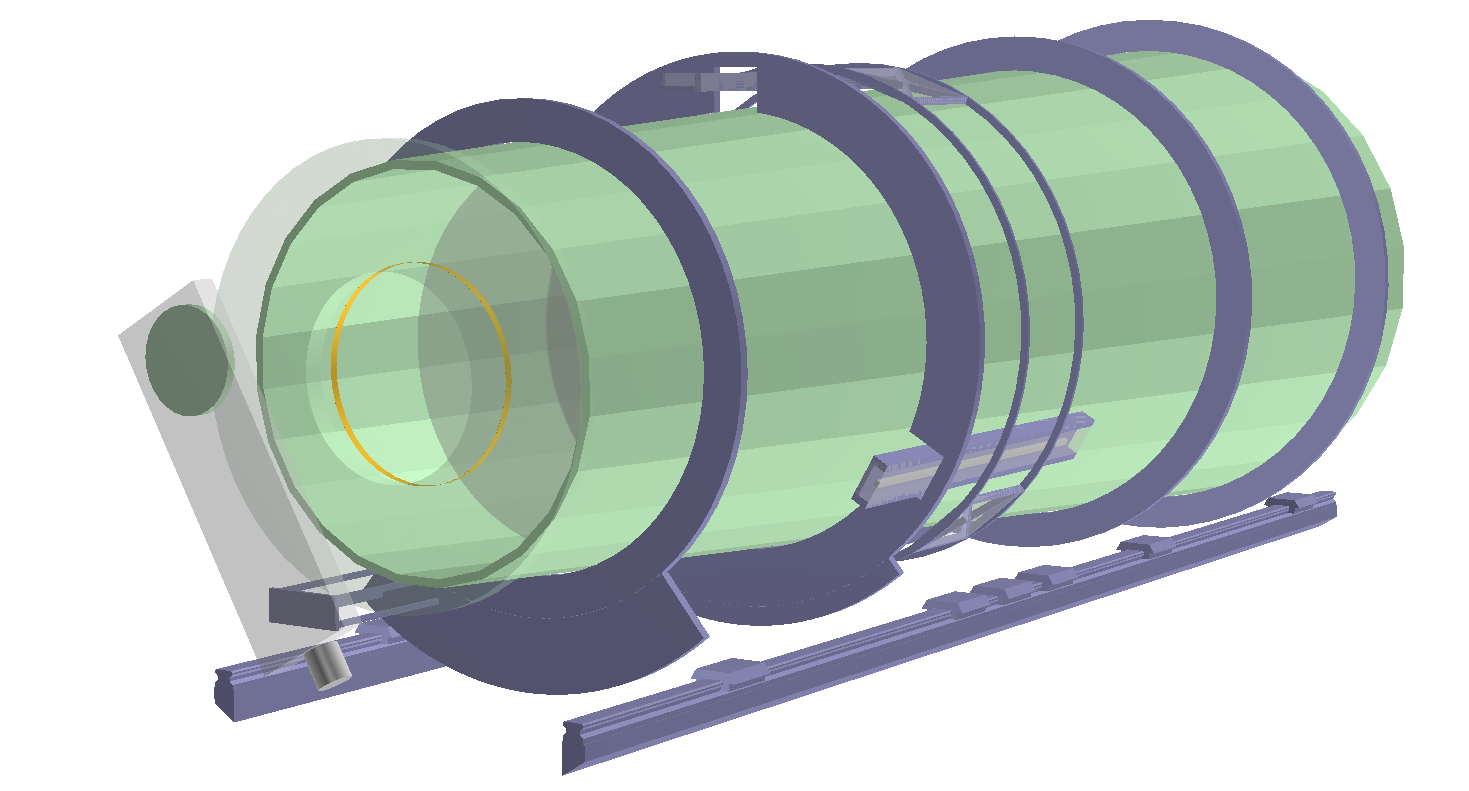
\includegraphics[width=0.90\textwidth]{png/pipenu_cele3b0_geom_degrader}
      }
    };
    % \node [text width=8cm, scale=1.0] at (14.5,0.5) {$\mu_B$, expected background mean};
    % \node [text width=8cm, scale=1.0, rotate={90}] at (1.5,7.5) { $S_{D}$, ``discovery'' signal strength  };
  \end{tikzpicture}
  \caption{
    \label{figure:degrader_v4}
    degrader v4: converter ring supported by OPA
  }
\end{figure}

%%%%%%%%%%%%%%%%%%%%%%%%%%%%%%%%%%%%%%%%%%%%%%%%%%%%%%%%%%%%%%%%%%%%%%%%%%%%%%
\subsection{Parameters used in the simulation}

\begin{itemize}
\item
  pion stops: reuse pipenu:bpim01b0, for the next iteration resimulate properly
\item
  converter thickness - 100$\mu$, width - 2 cm, $R_{out} = 250$ mm
\item 
  for simulating RPC photons: degrader material: CH2 , 24mm thick,
  to approximately match the material of 4mm thick Ti converter.
  May need to re-optimize the thickness to match the pion stopping rate
  at the ST to that of 4mm Ti
\item
  10M events $\gamma$ events, 
\item
  simulated range of cos(theta): [0,0.45] 
\item
  dataset family: rpc07b0
\end{itemize}

\begin{figure}[H]
  \begin{tikzpicture}
    \node[anchor=south west,inner sep=0] at (0,0.) {
      % \node[shift={(0 cm,0.cm)},inner sep=0,rotate={90}] at (0,0) {}
      \makebox[\textwidth][c] {
        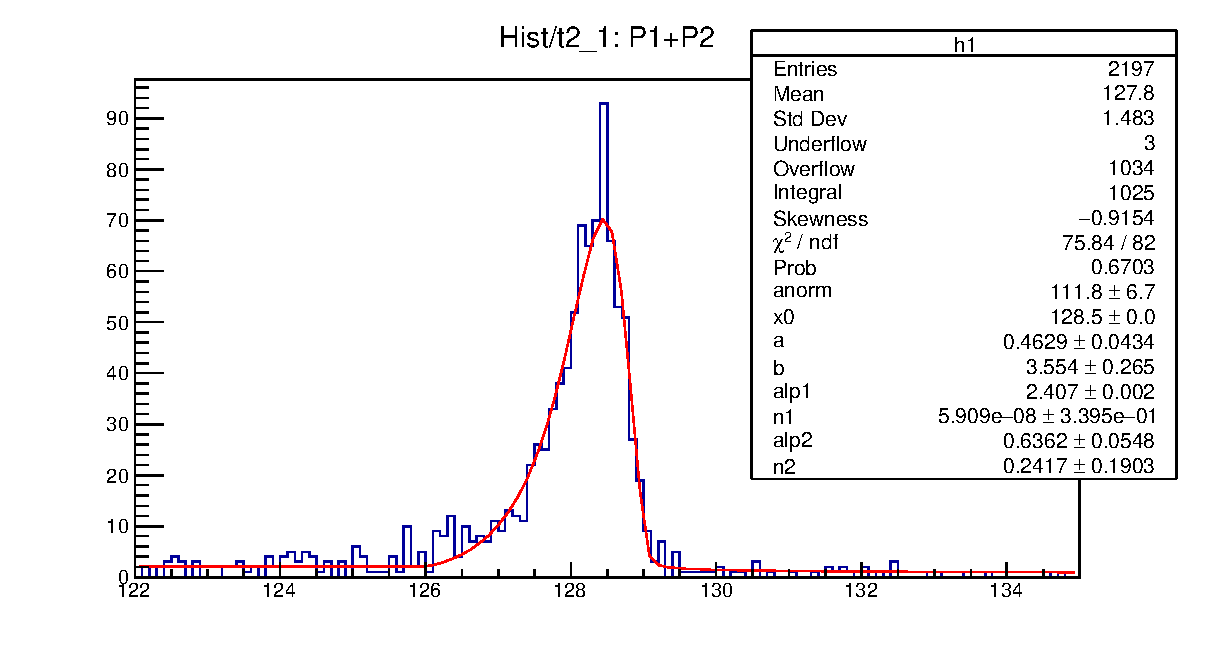
\includegraphics[width=0.95\textwidth]{pdf/pipenu_rpc07b0s51r0100_drpc_ana_t2_1_smom_1_fit}
      }
    };
    % \node [text width=8cm, scale=1.0] at (14.5,0.5) {$\mu_B$, expected background mean};
    % \node [text width=8cm, scale=1.0, rotate={90}] at (1.5,7.5) { $S_{D}$, ``discovery'' signal strength  };
  \end{tikzpicture}
  \caption{
    \label{figure:t2_1_smom_0}
    Sum of the two reconstructed track momenta and its fi.t 2cm wide converter in OPA
  }
  \label{figure:event_display}
\end{figure}

%%%%%%%%%%%%%%%%%%%%%%%%%%%%%%%%%%%%%%%%%%%%%%%%%%%%%%%%%%%%%%%%%%%%%%%%%%%%%%
\newpage
\subsection{Impact on the CE acceptance}

Figure~\ref{figure:ce_momentum_tsda} compares acceptances for the reconstructed CE tracks
got default geometry and geometry w/o the converter.
\begin{itemize}
\item 
  CE on Al for this comparison have been generated with the radiative corrections
  taken into account in the LL approximation.
\item 
  A model of perfect detector has been used - no misalignments, no miscalibrations.
\item
  2.5M events simulated per configuration.
\end{itemize}

Plotted in Figure~\ref{figure:ce_acceptance} are the momentum distributions for all
reconstructed CE tracks, w/o any selections applied. 

Comparison of the distributions tells that for the momentum window of [103,105] MeV/c,
an introduction of the Au converter reduces the CE acceptance by 0.16\%.

\begin{figure}[H]
  \begin{tikzpicture}
    \node[anchor=south west,inner sep=0] at (0,0.) {
      % \node[shift={(0 cm,0.cm)},inner sep=0,rotate={90}] at (0,0) {}
      % \makebox[\textwidth][c] {
        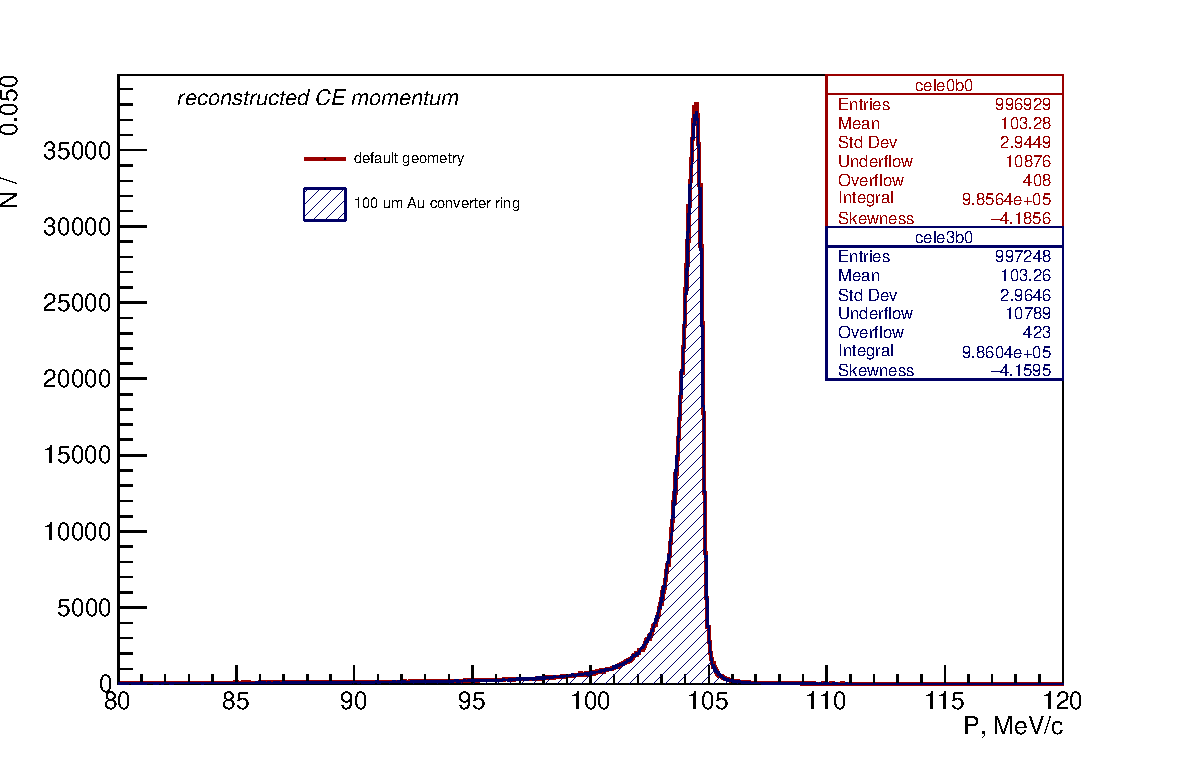
\includegraphics[width=0.54\textwidth]{pdf/figure_00051}
      % }
    };
    \node[anchor=south west,inner sep=0] at (9.8,0.) {
      % \node[shift={(0 cm,0.cm)},inner sep=0,rotate={90}] at (0,0) {}
      % \makebox[\textwidth][c] {
        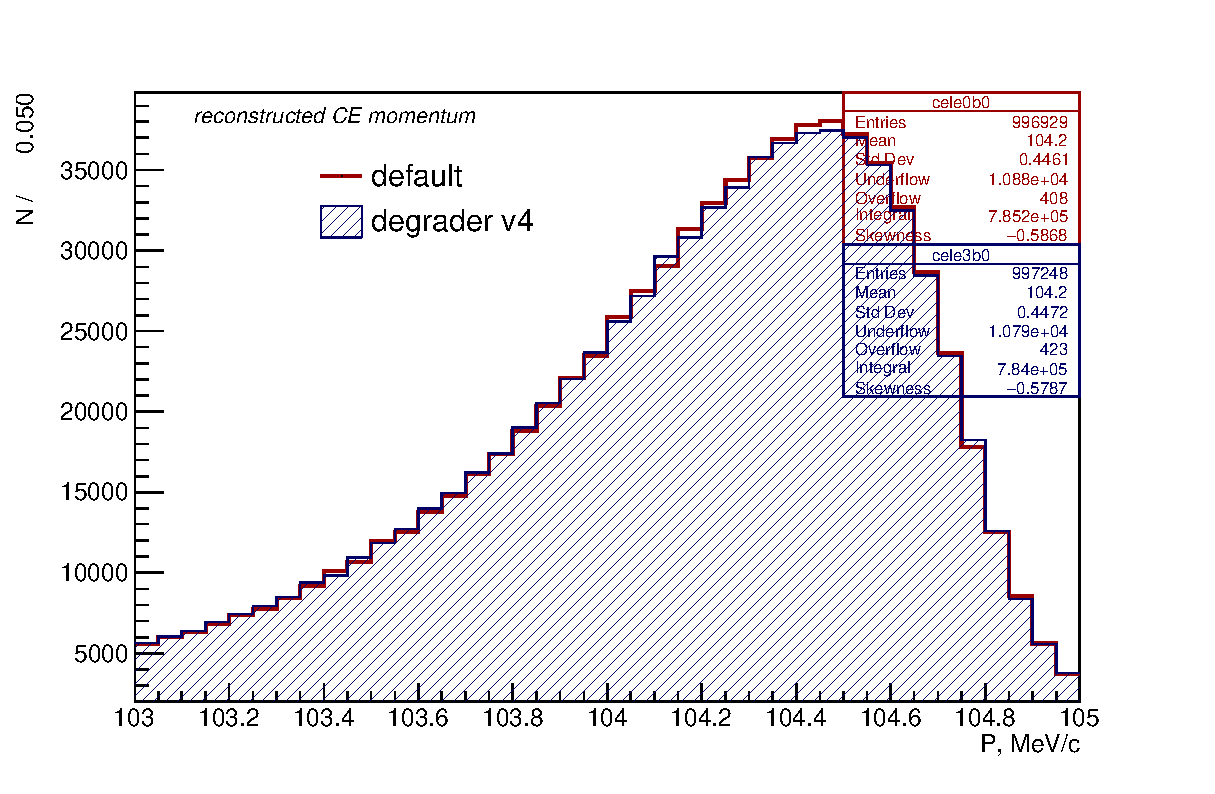
\includegraphics[width=0.54\textwidth]{pdf/figure_00052}
      % }
    };
    % \node [text width=8cm, scale=1.0] at (14.5,0.5) {$\mu_B$, expected background mean};
    % \node [text width=8cm, scale=1.0, rotate={90}] at (1.5,7.5) { $S_{D}$, ``discovery'' signal strength  };
  \end{tikzpicture}
  \caption{
    \label{figure:ce_acceptance}
    CE momentum distribution for two geometries, with and without the converter ring. 
  }
  \label{figure:ce_momentum_tsda}
\end{figure}
%%% Local Variables:
%%% mode: latex
%%% TeX-master: t
%%% End:
